\chapter{Choosing Industries for Wealth Creation}

The exchange begins with a narrow question that carries a broad entrepreneurial problem: if the aim is to create wealth, where should a person look first? The speaker answers with a ranked sequence rather than a theory of everything. Real estate comes first because it is presented as accessible. Technology comes second because it can create wealth but demands judgment. The third answer, an industry one already knows, closes the loop by turning familiarity into a practical risk filter.

\paragraph{Source note.}
This chapter follows a School of Hard Knocks entrepreneurship interview curated for the LazyEarn track by LazyingArt LLC through Video2Book. The primary evidence is the spoken interview.

\section{The Opening Wealth Question}

The interviewer asks for the best three industries people should be looking at in order to create wealth in today's world. That is the organizing question. It is not asking for a single business model, a financing tactic, or a motivational rule. It asks us to choose the field of play.

That distinction matters. Before we decide what to sell, how to fund it, or how to scale it, we need to ask whether the arena itself rewards the kind of learning, capital, and judgment we can bring to it. The speaker's answer is short, but it has a sequence: access first, discernment second, familiarity third.

\subsection{Question \& Answer}

\paragraph{Question.}
What are the best three industries for someone trying to create wealth today?

\paragraph{Answer.}
The speaker gives a ranked answer:

\begin{enumerate}
\item Real estate.
\item Technology.
\item An industry that you already know something about.
\end{enumerate}

The useful point is not only the list, but the order. We begin with a market the speaker sees as enterable, then move to a field where upside is mixed with danger, and finally return to the learner's own base of knowledge.

\begin{figure}
\centering
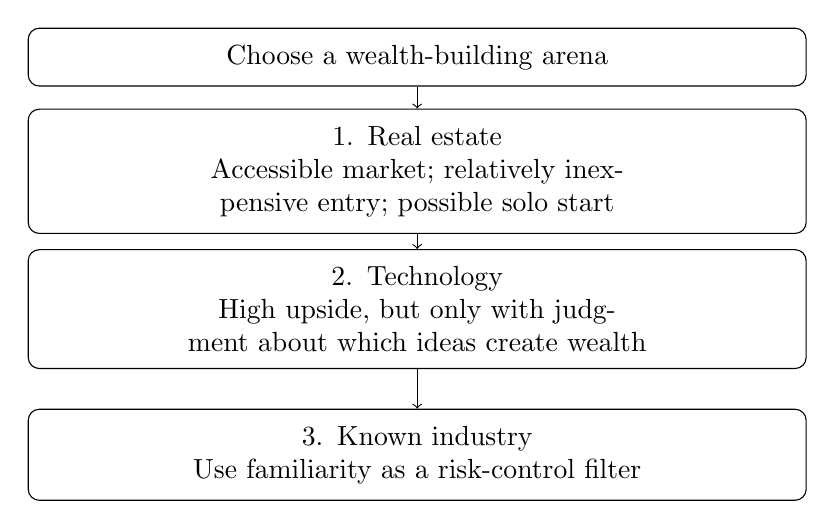
\begin{tikzpicture}[
  every node/.style={
    draw,
    rounded corners,
    align=center,
    text width=0.78\linewidth,
    inner sep=6pt
  }
]
\node (q) at (0,0) {Choose a wealth-building arena};
\node (r) at (0,-1.45) {1. Real estate\\Accessible market; relatively inexpensive entry; possible solo start};
\node (t) at (0,-3.20) {2. Technology\\High upside, but only with judgment about which ideas create wealth};
\node (k) at (0,-5.05) {3. Known industry\\Use familiarity as a risk-control filter};
\draw[->] (q) -- (r);
\draw[->] (r) -- (t);
\draw[->] (t) -- (k);
\end{tikzpicture}
\caption{A compact reconstruction of the spoken ranking. The sequence moves from access, to judgment, to familiarity.}
\end{figure}

\section{Real Estate: Access First}

The first answer is real estate. The speaker calls it a fantastic market and says one can get into it relatively inexpensively and do it by oneself.

\paragraph{Claim.}
Real estate is presented as a strong wealth-building arena.

\paragraph{Mechanism.}
The mechanism is access. The speaker does not dwell on leverage, property cycles, tax treatment, or institutional investing. He points instead to the possibility of beginning without a large apparatus. In these notes, that is the reason real estate comes first: it answers the beginner's problem of entry.

\begin{definition}[Accessible entry]
An industry has accessible entry when a beginner can plausibly begin learning and operating without first needing a large team, a specialized technical staff, or control of a large institution.
\end{definition}

This is not a formal law. It is a practical reading of the speaker's emphasis. A market can be large and still be a poor starting point if the first step is too expensive, too opaque, or too dependent on permission from others. The real-estate recommendation is framed in the opposite way: one can begin, learn, and operate.

\section{Technology: Upside With a Warning}

The second answer is technology, but it arrives with a caution attached. The speaker says one really needs to know a lot about technology as it relates to which technologies will propel wealth and which may suck wealth.

That is the turn in the lecture. Real estate is introduced through access. Technology is introduced through discernment. The problem is not that technology lacks opportunity. The problem is that opportunity and waste can look similar when we do not understand the field.

\begin{remark}
The phrase ``suck wealth'' should be read as a commercial warning. A bad opportunity can consume capital, attention, time, and credibility even when it sounds modern or exciting.
\end{remark}

The technology recommendation therefore has two sides:

\begin{itemize}
\item Technology can be a wealth-building field.
\item Technology requires judgment about which ideas are actually capable of creating wealth.
\end{itemize}

If we preserve only the first statement, we make the advice too broad. If we preserve both, the recommendation becomes more precise: technology is attractive only when the entrepreneur can evaluate it.

\section{The Filtering Problem}

The speaker says there are a lot of great technology ideas, and even more terrible ones. This is the central filter problem. The category name is not enough. We have to sort inside the category.

A compact table helps keep the logic visible without pretending that the interview supplied a numerical model.

\begin{table}
\centering
\begin{tabular}{p{0.28\linewidth} p{0.62\linewidth}}
\hline
Industry & Claim and filter \\
\hline
Real estate & Strong market; relatively inexpensive entry; possible to begin alone. The filter is whether the learner can start operating without excessive complexity. \\
Technology & Potential wealth builder, but only with enough knowledge to distinguish strong ideas from dangerous ones. The filter is judgment. \\
Known industry & Recommended because prior familiarity improves the first round of decision-making. The filter is what the learner already understands. \\
\hline
\end{tabular}
\caption{Transcript-derived selection logic. The table is a compact reading aid, not a scoring formula.}
\end{table}

\paragraph{A worked selection check.}
Suppose we are comparing three possible starting points: a small real-estate operation, a technology idea we do not understand, and a business in a field where we already have experience. The speaker's logic does not tell us to choose the most fashionable option. It tells us to test the options in order.

\begin{enumerate}
\item Ask whether the field is enterable: can we begin learning and operating without excessive cost or institutional dependence?
\item If the field is technology, ask whether we understand why this idea should propel wealth rather than consume it.
\item Ask whether we already know enough about the industry to recognize customers, normal problems, hidden costs, and weak assumptions.
\end{enumerate}

Under this check, an unknown technology idea is not automatically rejected. It simply cannot pass on novelty alone. It needs evidence and judgment. The familiar industry may be less glamorous, but it can be a better starting point because the entrepreneur has a map, even if it is incomplete.

\section{An Industry You Know}

The third answer is an industry that one already knows something about. The speaker makes the threshold deliberately modest: whether it is a little or a lot, get into something already familiar.

This resolves the earlier warning about technology. If there are many terrible ideas mixed among the good ones, then prior knowledge becomes a way of seeing. It helps the entrepreneur notice what outsiders miss: how customers behave, where costs hide, which promises are unrealistic, and what a real problem looks like before it becomes a pitch deck.

\begin{definition}[Familiarity filter]
The familiarity filter is the discipline of preferring arenas where the entrepreneur already has some direct knowledge. It does not replace research, but it improves the first round of judgment.
\end{definition}

The point is not to stay forever inside what is already comfortable. The point is to avoid beginning from total blindness. A little familiarity can make the first questions better, and better questions can prevent expensive mistakes.

\section{Summary: Access, Judgment, Familiarity}

The interview gives a short ranked list, but the list is held together by a practical sequence. Real estate appears first because it is framed as accessible. Technology appears second because it can create wealth, but only when the entrepreneur can distinguish strong ideas from weak ones. A known industry appears third because familiarity reduces the danger of blind entry.

The durable lesson is that wealth creation begins with arena selection. We choose where to play before we choose the exact move. The speaker's order gives us a compact discipline: start where entry is possible, respect the need for judgment, and use familiarity as a filter against chasing opportunities we do not yet understand.